\chapter{Introduction}
\label{ch:introduction}
The use of scientific computing to studying the Qur'\=an is still in its early stage in the fields of Islamic Studies and Statistical and Machine Learning applications. This study will therefore benefit not only the researchers from Islamic Studies but also Statisticians and Machine Learning practitioners who are into text analytics. Having said that, it is therefore necessary to provide context to audiences of these disciplines to provide background on the state of Qur'\=anic studies and the increasing adoption of scientific methodology to studying humanities.
\section{Background}
The Qur'\=an or \arb[trans]{al-qur'An} \arb{al-qur'An} meaning \textit{the recitation}, the holy book of Islam, is revered by 1.9 billion (according to 2020 projection of \shortciteA[p.~13]{pewresearch}) Muslims across the globe as the literal words of God. Muslims believed that the Qur'\=an was gradually revealed (Qur'\=an 25:32) to Prophet Muhammad \arb{\arbmark{slm}} through angel \arb[trans]{jibrIl} \arb{jibrIl} or Gabriel (Qur'\=an 2:97). The Qur'\=an contains 77,429 Arabic words in total, which covers only 56 percent of the Greek New Testament which has 138,020 words in total \cite[p.~11]{sinai2017}. 

The Qur'\=an is divided into \arb[trans]{sUwar} \arb{sUwar} (\textit{plural} of \arb[trans]{sUraT} \arb{sUraT}) which are the equivalent of chapters, each containing \arb[trans]{'AyAt} \arb{'AyAt} (\textit{plural} of \arb[trans]{'AyaT} \arb{'AyaT} meaning \textit{signs}), which are the equivalent of verses. The \arb[trans]{sUwar} \arb{sUwar} are not arranged in chronological order as in the Bible's books and chapters, but rather arranged in monotonically decreasing length of number of verses after the first \arb[trans]{sUraT} \arb{sUraT} (\textit{see} Figure \ref{fig:ayah_word_count}). The \arb[trans]{sUwar} \arb{sUwar} of the Qur'\=an can be categorized into two types: the \arb[trans]{makkiyyaT} \arb{makkiyyaT} (Meccan) and \arb[trans]{madaniyyaT} \arb{madaniyyaT} (Medinan). The categories refer to the geographical location of where the \arb[trans]{sUraT} \arb{sUraT} was revealed. Figure \ref{fig:ayah_word_count} shows the grouping of the \arb[trans]{sUwar} \arb{sUwar}. Note that some of the \arb[trans]{sUwar} \arb{sUwar} have mixed geographical locations\footnote{\textit{see} list of the location in \url{https://tanzil.net/docs/revelation_order}}, that is, a few of the \arb[trans]{'AyAt} \arb{'AyAt} in it were revealed in other geographical location apart from the geographical location of the rest of the \arb[trans]{'AyAt} \arb{'AyAt}. Therefore, the categorization in Figure \ref{fig:ayah_word_count} highlights the geographical location of the majority of the \arb[trans]{'AyAt} \arb{'AyAt} in the \arb[trans]{sUraT} \arb{sUraT}.

\begin{figure}[!b]
    \centering
    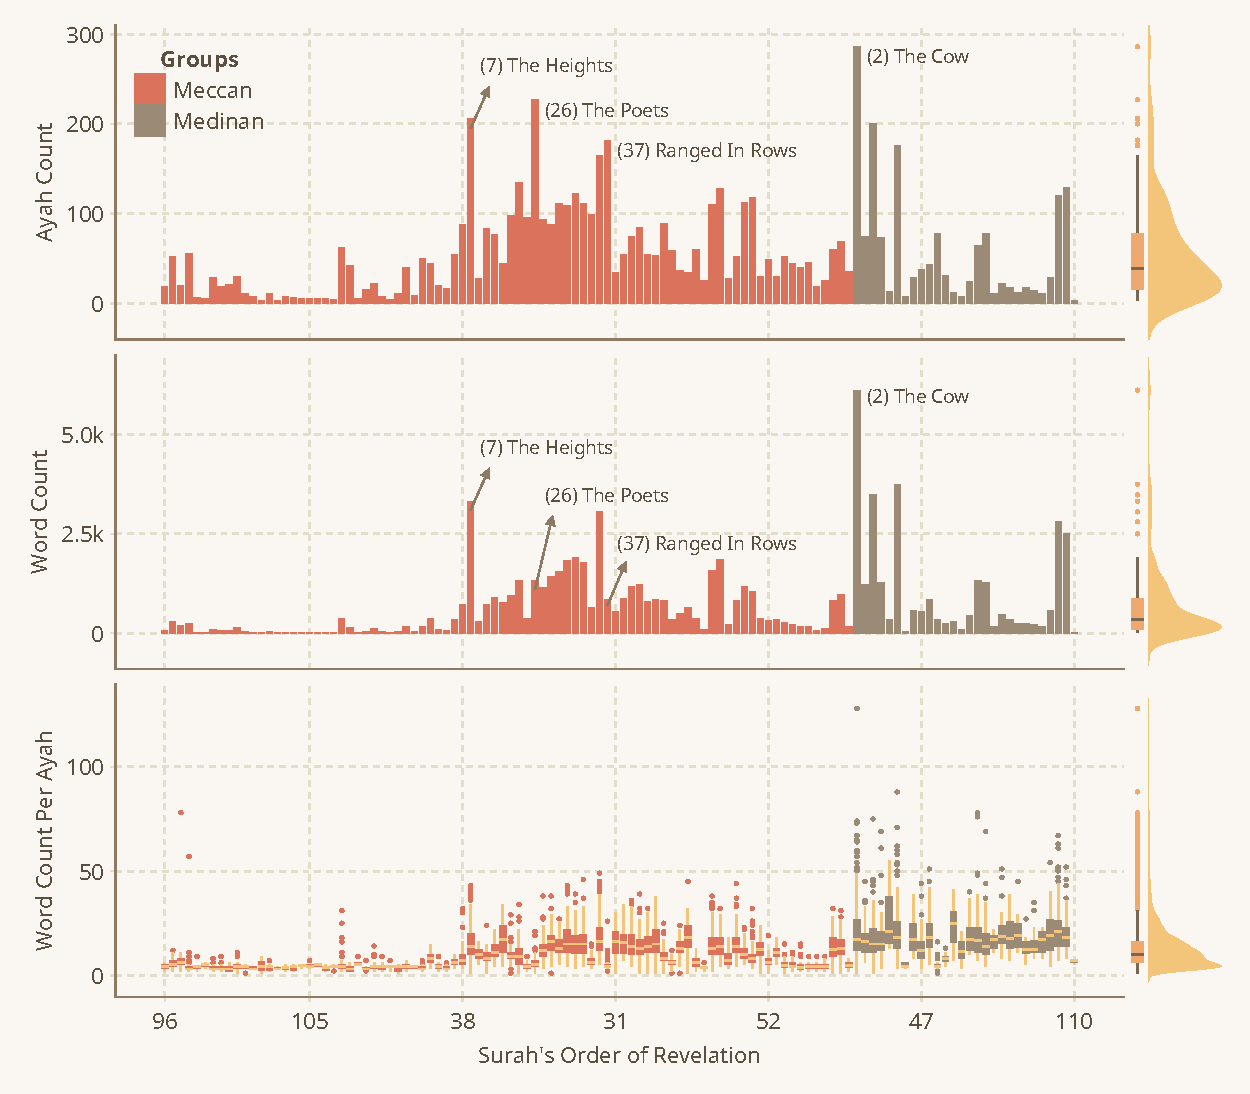
\includegraphics[width=\textwidth]{img/plot2.pdf}
    \caption{Statistics of the words and \arb[trans]{'AyAt} \arb{'AyAt} (verses) of the Qur'\=an}
    \label{fig:ayah_word_count}
\end{figure}

\section{Rationale of the Study}\label{sec:rationale}
Attempts at understanding the Qur'\=an by Qur'\=anic scholars were mostly done with the use of manual processes, that is, studying the scriptures by going through its content one-at-a-time manually. However, with the advent of computers, some researchers have started using it to aid in their study. The first known to have used computers for studying the Qur'\=an was likely Rashad Khalifa in 1968\footnote{\url{https://www.masjidtucson.org/quran/miracle/a_profound_miracle_sura68nun133.html}}, where he studied the significance of the mysterious initials at the beginning of some \arb[trans]{sUwar} \arb{sUwar}. Rashad uploaded the Qur'\=an into his computer by transliterating the Arabic letters and other Qur'\=anic orthographies into Roman letters and symbols that the computer can easily parse. This approach of using computers to find new insights is more common in the field of science, and it was new to the field of Qur'\=anic studies.

Indeed, to proceed with the use of scientific computing, the Qur'\=an will be treated as the data that needs to be analyzed using what is called Natural Language Processing (NLP), a branch of Machine Learning (ML) that aims to understand natural languages, such as Arabic. To instruct the computer to do Statistical analyses, ML, or NLP, one needs to use a \textit{software application} or a formal language called \textit{programming language}. There are several programming languages that the computer can understand. The popular one for researchers in the field of sciences are Python \cite{van1995python}, R \cite{rprogramming}, and sometimes Julia \shortcite{Julia2017}. These programming languages will be used to construct instructions for computer. Therefore, if the data is the Qur'\=an, then there should be a way to interface with it using any of these programming languages. Or alternatively, there should be a way to upload it into the chosen programming language and encode the Arabic letters into something that can be easily parsed by the computer, like what Rashad \mbox{Khalifa} did. Having said that, there are indeed some programming languages with libraries or packages for interfacing with the Qur'\=an, and this is true for Python, R, and \mbox{Julia}. For this study, Julia programming language will be used for interfacing with the Qur'\=an texts since its library for it has more features \cite<\textit{see}>{asaad2021qurantree} compared to R and Python. The said Julia library is the QuranTree.jl\footnote{\url{https://alstat.github.io/QuranTree.jl/stable/}}. QuranTree.jl is based on Tanzil\footnote{\url{https://tanzil.net/download/}} for the Qur'\=anic Arabic texts, and \citeA{dukes-habash-2010-morphological} for morphological annotation, which both libraries from R and Python do not have in terms of morphological annotation from \citeA{dukes-habash-2010-morphological}. However, both R and Python will still be used for this paper for libraries that are not available in Julia. In particular, R is known for niche statistical libraries since it was made for statistical computation, whereas Python is now popular for Deep Learning frameworks for complex modeling like TensorFlow\footnote{\url{https://www.tensorflow.org/}} (a library made by Google\footnote{\url{https://research.google/}}) and PyTorch\footnote{\url{https://pytorch.org/}} (a library made by Meta\footnote{\url{https://ai.meta.com/}}). 

Now that the programming languages for this paper have been identified, next is to understand how Statistics and Machine Learning can help in studying the Qur'\=an. Statistics is a branch of Science that aims to study features or characteristics of data generated from a random phenomenon. The findings of Statistical analyses can then be used to make conclusions or predictions of the general population of the data or general characteristics of the data. Machine Learning or ML, on the other hand, is a branch of Artificial Intelligence that heavily intersects with Statistics, albeit with distinct differences as well. Both Statistics and ML aims to characterize data by learning its features, but ML researchers have been aiming on complex models that are often inspired by simpler models from Statistics. Therefore, one can think of Statistics as one of the fundamentals of ML. 

One of the goals of Statistics and Machine Learning is to summarize all of the learned features into a hypothesized equation or hypothesized mathematical formula whose parameters or weights are optimized to capture the most characteristics of the data. It is called hypothesized equation since the researcher is the one who decide which family of equation best describe the characteristics of the data. The said equation is called a \textit{model}. Therefore, a model is a generic entity that can be fitted or molded to capture the features of the data. Mathematically and in general, a model can be related to the data as:
\begin{equation}\label{eq:general_model}
    y:=h(x|\boldsymbol{\theta})+\varepsilon,
\end{equation}
where $h(x|\boldsymbol{\theta})$ is the hypothesized model taking the input data $x$, where $x\in\mathscr{X}$, and outputs a target data $y$, where $y\in\mathscr{Y}$. Therefore, $h:\mathscr{X}\rightarrow\mathscr{Y}$. The $\varepsilon$ is the error that the hypothesized model $h(x|\boldsymbol{\theta})$ cannot capture even after finding the best configuration of its parameter $\boldsymbol{\theta}$. Therefore, ideally the error or \textit{residual} or sometimes called \textit{innovation}, $\varepsilon$, should exhibit a \textit{random noise} for us to say that the hypothetical model $h(x|\boldsymbol{\theta})$ has captured well the core characteristics of the data $(x,y)$. These random noise are data points that could have come from other factors that are not available in the given data, $(x,y)$. Therefore, the idea of modeling is to find the optimal value of $\boldsymbol{\theta}$ in such a way it will minimize the error between the actual data (represented by $y$ below) and the predicted one $\hat{y}$:
\begin{equation}
    \varepsilon:=y-\hat{y}=y-h(x|\boldsymbol{\theta}).
\end{equation}

To help understand the concept of modeling, and relate it to the fashion industry, which the author assumes most readers are familiar with, a model in a fashion industry is responsible for representing the characteristics of the target customers (in Eq. \ref{eq:general_model} this is $y$). Therefore, for a clothing company, they hire Asian models (in Eq. \ref{eq:general_model}, this is $h(x|\boldsymbol{\theta})$) to target Asian customers (in Eq. \ref{eq:general_model} this is $y$). So that, when these models wore the clothes sold by the said company, the potential customer will more or less be able to relate to the model, and be able to imagine themselves wearing that same clothes as well, which help them incline to buying the said clothing. The model, therefore, does not necessarily have the looks of every target Asian customers, but at least in terms of height, skin tone, hair, and other common Asian features, the model will likely have it, or at least the difference is more or less minimal (in Eq. \ref{eq:general_model}, the difference is represented by $\varepsilon:=y-\hat{y}$). The question now is, what are the benefits that this model can bring to the clothing company? Well, the clothing company will be able to create products that are tailored to their Asian customers using the said model, since the company will have the right baseline measurements needed. Relating this analogy to the technical concept discussed earlier, you can think of the target customers as the
real or actual data (in Eq. \ref{eq:general_model} this is $y$), and the model as the same technical term use in Machine Learning and Statistics (in Eq. \ref{eq:general_model} this is $h(x|\boldsymbol{\theta})$), but this time this technical model is expected to capture the characteristics of the real data analogous to fashion model that is expected to capture the characteristics of the target customer. This Statistical or Machine Learning model brings the following benefit: researchers will be able to study the real data by simply using the model to answer questions that are not available in the sampled real data.

Having understood what models are, let's turn our attention to the objectives of this paper. The aim of this paper is to make use of the Statistical or Machine Learning modeling to understand the characteristics of the Qur'\=an. More specifically, the next section will list down the research questions of this paper.

\section{Objectives}\label{sec:objectives}
The following are the general and specific objectives of this paper:
\begin{enumerate}
    \item What are the structural characteristics of the Qur'an that can be extracted from its rich morphologies using statistical and large language models?
    \begin{enumerate}
        \item What are the statistics of the Qur'\=an's morphological features in terms of its parts of speech and selected entities like God's name and the prophets names mentioned?
        
        \item How do the rhythmic signatures of the Qur'\=an of the verses looks like and what are statistical insights that can be extracted?
        
        \item What are the supporting statistical insights on the current divisions of the Qur'\=an's verses? 
    \end{enumerate}
    
    \item What other insights that can be extracted from the semantics of the Qur'an's texts using statistical and large language models?
    \begin{enumerate}
        \item How does the theory of \textit{concentrism} be formulated statistically, and what are the insights from the statistical and large language models on this? 
        
        \item How do the surahs are organized in terms of the topics? What are the themes that can be extracted for each of the surahs?
        
        \item How do these extracted themes compare to the summaries of Abdel\linebreak Haleem's English translation of the Qur'an?
    \end{enumerate}
    
    \item How does this combination of statistical, machine learning, and artificial intelligence with the Muslim's traditional literatures help in understanding the Qur'\=an, especially with the advent of Generative AI?
\end{enumerate}

\section{Significance of the Study}\label{sec:significance}
While the Qur'\=an has been extensively studied by Muslims and non-Muslims scholars alike, especially in the topic of Meccan and Medinan surahs, there is still a lot to uncover from the perspective of Computational Statistics. Hence, the significance of this study is that it brings forward new ways of extracting insights from the Qur'\=an by leveraging Computations, Statistics, Machine Learning, and AI, that is still in its early stage in the field of Qur'\=anic Studies. Therefore, this new perspective or process of studying the scripture not only aids the scholars of the Islamic Studies, but may also contribute indirectly to community development and policy makers who use Qur'\=an as part of their decision making.
\section{Scope of the Study}
The paper will cover all chapters of the Qur'\=an both for the Morphological and Topic Modeling analyses, but it will only present the results of \textit{s\=urahs} \arb{sUr} with at least 1000 words. The rest of the result will be part of the web application that can be used to query the Qur'\=an. It will also not delve into the \textit{tafsir} \arb{tafsIr} of each of the verses, but only when necessary for further context.
\section{Thesis Organization}
The paper is organized as follows: Chapter 2 will discuss the related literatures, Chapter 3 will discuss the methodology, Chapter 4 will present the results and discussions, and finally Chapter 5 will contain the conclusion and recommendation. The references and appendices are placed after the Chapter 5.